\documentclass[citation\_needed]{subfiles}
\begin{document}

SEM\footnote{dont une interface web est disponible à l'adresse suivante : \url{http://apps.lattice.cnrs.fr/sem/}} \citep{tellier2012segmenteur,dupont2014reconnaisseur} est un outil dont j'ai commencé le développement en licence au sein de l'Université d'Orléans et poursuivi depuis. Il permet d'effectuer diverses tâches d'étiquetage, notamment en Part-Of-Speech, chunking et entités nommées. Il utilise un CRF pour effectuer l'annotation, plus précisément Wapiti \citep{lavergne10} et a été entrainé sur le French Treebank \cite{Abeille03,sagot2012annotation}.

SEM permet d'enchainer un ensemble de traitements (pipeline) simples pour effectuer des tâches complexes (voir figure\ \ref{fig:sem-pipeline}), le rendant très configurable. Une illustration des traitements effectués par SEM pour effectuer du chunking est disponible dans la figure\ \ref{fig:sem-pipeline-showcase}. Cela lui permet de traiter autant du texte brut qu'il peut segmenter en tokens et phrases, ou des fichiers au format CoNLL (tabulaires). En plus de sa capacité à enchainer les traitements, une force de SEM est qu'il offre la possibilité de décrire des traits à calculer afin d'enrichir les données en entrée. Ces traits sont décrits à l'aide un langage XML, évitant ainsi l'effort de devoir les coder directement. Ce processus permet l'ajout de nombreux traits de façon très simple et configurable. Les traits définis dans SEM utilisent autant des expressions régulières (vérification, sous-séquence, substitution, etc.), des expressions booléennes, des dictionnaires de tokens et de séquences de tokens, ainsi que le séquencage de traitements (par exemple une suite de substitutions). Un exemple de fichier annoté et exporté au format HTML est donné dans la figure\ \ref{fig:sem-html} (en annexe, un exemple de fichier d'enrichissement de SEM est également donné en figure\ \ref{fig:sem-features}).

SEM dispose de plusieurs modules pouvant s'appeler soit indépendamment soit de manière groupée dans une pipeline, l'idée étant de pouvoir effectuer autant des traitements spécifiques, comme par exemple tester un nouveau jeu de traits sur un corpus au format CoNLL, que des traitements plus généraux, comme prendre un fichier de texte brut et le traiter jusqu'à l'annotation en entités nommées. Les modules principaux de SEM sont les suivants:
\begin{itemize}
    \item tagger : le module principal de SEM. Il permet d'enchaîner les traitements divers selon une pipeline.
    \item segmentation : le module pour effectuer la segmentation. Il recourt à des objets segmenteurs qui calculents les frontières entre les différents éléments (tokens, phrases, paragraphes). Il existe actuellement un segmenteur pour le Français et un pour l'Anglais. Ces segmenteurs sont retrouvés de façon nominative, ainsi, l'intégration d'un nouveau segmenteur demande juste l'ajout d'un fichier source dans le bon dossier (le code doit, évidemment, respecter certaines règles)
    \item enrich : le module pour ajouter des features à un corpus au format CoNLL. Il recourt à un ensemble "d'enrichisseurs", qui sont des objets effectuant un traitement très basique (comme évaluer si l'on est en début de phrase) compilés depuis un langage XML tel qu'illustré sur la figure\ \ref{fig:sem-features}.
    \item label : effectue l'annotation du corpus à l'aide de Wapiti.
    \item export : le module pour l'écriture en sortie des résultats, il suit la même philosophie que le module de segmentation pour retrouver les objets dit "exporteurs". Les formats supportés actuellement sont : texte linéaire, texte tabulaire et HTML. Il est prévu d'intégrer le support du XML-TEI pour pouvoir être importé dans ANALEC \citep{landragin2012analec}.
\end{itemize}

\begin{savenotes}
\begin{table}[ht!]
\centering
\begin{tabular}{|l|ccc|}
\hline
tâche    & précision & rappel & f-mesure \\
\hline
POS      & 97.7      & 97.7   & 97.7 \\
chunking\footnote{les résultats en termes de précision et rappel n'ont pas été publiés et furent perdus par la suite} & ?         & ?      & 97.53 \\
NER      & 84.07     & 77.47  & 80.64 \\
\hline
\end{tabular}
\caption{les chiffres de qualité de SEM sur les différentes tâches}
\end{table}
\end{savenotes}

\begin{figure}[ht!]
\centering
\includegraphics[scale=0.5]{images/SEM/html-example}
\caption{exemples de sortie de SEM}
\label{fig:sem-html}
\end{figure}

\begin{figure}[ht!]
\centering
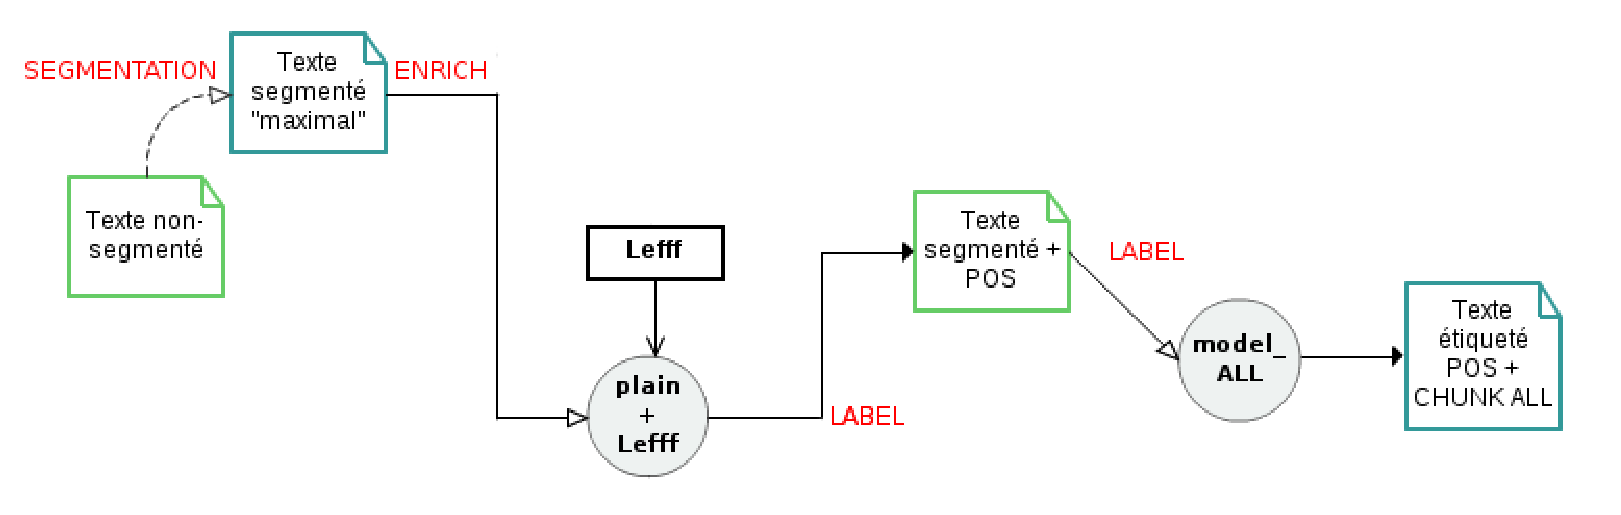
\includegraphics[scale=0.5]{images/SEM/pipeline-example}
\caption{illustration d'une chaine de traitement de SEM}
\label{fig:sem-pipeline-showcase}
\end{figure}

\end{document}